%% LyX 1.6.4 created this file.  For more info, see http://www.lyx.org/.
%% Do not edit unless you really know what you are doing.
\documentclass[10pt,a4paper,english]{article}
\usepackage{avant}
\renewcommand{\familydefault}{\sfdefault}
\usepackage[T1]{fontenc}
\usepackage[latin9]{inputenc}
\usepackage{listings}
\usepackage{fancyhdr}
\pagestyle{fancy}
\usepackage{babel}

\usepackage{varioref}
\usepackage{float}
\usepackage{framed}
\usepackage{graphicx}
\usepackage[unicode=true, 
 bookmarks=true,bookmarksnumbered=false,bookmarksopen=false,
 breaklinks=false,pdfborder={0 0 0},backref=false,colorlinks=false]
 {hyperref}
\hypersetup{pdftitle={ROSA - Real time Operating System for AVR32},
 pdfauthor={Marcus Jansson}}
 
\makeatletter
%%%%%%%%%%%%%%%%%%%%%%%%%%%%%% Textclass specific LaTeX commands.
\newenvironment{lyxcode}
{\par\begin{list}{}{
\setlength{\rightmargin}{\leftmargin}
\setlength{\listparindent}{0pt}% needed for AMS classes
\raggedright
\setlength{\itemsep}{0pt}
\setlength{\parsep}{0pt}
\normalfont\ttfamily}%
 \item[]}
{\end{list}}

\makeatother

\begin{document}

\title{ROSA}


\author{Marcus Jansson <mjansson256@yahoo.se>}
\maketitle
\begin{lyxcode}
\begin{center}
{\Large A~tiny}
\par\end{center}{\Large \par}

\begin{center}
{\Large Real~time~Operating~System~for~AVR32}
\par\end{center}{\Large \par}

\begin{center}
\pagebreak{}
\par\end{center}

\tableofcontents{}\pagebreak{}
\end{lyxcode}

\section{Description}

ROSA is a small cooperative real time kernel for AVR32 UC3A processors.
It is aimed to be used on the Atmel EVK1100 platform.

This document is a description of ROSA's support for pseudo parallel
execution of user programs. By {}``pseudo parallel'' we mean it
{}``seems'' like the programs work in parallel. But as the UC3A
processor is a single core processor, only one program at a time can
be executed.

A small operating system like ROSA can be used to enhance the structure
of a complex program. This is done by breaking down the complex program
into several smaller programs.

Compared to other light weight kernels, ROSA is a tiny kernel with
very limited functionality.


\subsection{Hardware}

ROSA runs on the EVK1100 platform. Among other things the hardware
features 512 kB flash memory, 64 kB internal RAM memory, a 12 Mhz
external crystal, user LEDs, user buttons, serial communication etc.


\subsubsection{I/O drivers}

ROSAs I/O drivers support the following hardware functions on EVK1100:
\begin{itemize}
\item LEDs.
\item Buttons.
\item Mini-joystick.
\item Potentiometer.
\item Serial port.
\end{itemize}

\subsection{Software}


\subsubsection{ROSA source code}

The ROSA source code is available in the rosa/src directory which
makes it possible to expand ROSA with more services. Examples of expansions
that can be done:
\begin{itemize}
\item Support for time sharing.
\item Support for priority driven scheduling.
\item Support for communication mechanisms, semaphores, monitors, mailboxes
and rendez-vouz.
\item ...
\end{itemize}

\subsubsection{Directory structure}

The ROSA software consists of the following directories and files:
\begin{itemize}
\item rosa/

\begin{itemize}
\item bin/\qquad{}\hfill{}- Destination for the binary files.
\item cpu/\qquad{}\hfill{}- The startup and linker scripts.
\item doc/\qquad{}\hfill{}- Documentation about ROSA.
\item include/\qquad{}\hfill{}- The header file directory.

\begin{itemize}
\item drivers/\qquad{}\hfill{}- Header files for the drivers.
\item kernel/\qquad{}\hfill{}- Header files for the kernel.
\end{itemize}
\item src/\qquad{}\hfill{}- The source file directory.

\begin{itemize}
\item main.c\qquad{}\hfill{}- The main program for ROSA.
\item rosa\_config.h\qquad{}\hfill{}- User configuration of ROSA.
\item kernel/\hfill{}- Kernel source directory.

\begin{itemize}
\item rosa\_ker.c\qquad{}\hfill{}- Kernel C source.
\item rosa\_ker\_asm.S\qquad{}\hfill{}- Kernel assembler source.
\item rosa\_scheduler.c\qquad{}\hfill{}- Scheduler specific source.
\item rosa\_int.c\qquad{}\hfill{}- Interrupt specific source.
\item rosa\_int\_asm.S\qquad{}\hfill{}- Interrupt assembler source.
\item rosa\_tim.c\qquad{}\hfill{}- Timer specific soruce.
\item rosa\_tim\_asm.S\qquad{}\hfill{}- Timer assembler source.
\end{itemize}
\item drivers/

\begin{itemize}
\item button.c\qquad{}\hfill{}- Push button driver.
\item delay.c\qquad{}\hfill{}- Delay functions.
\item gpio.c\hfill{}- GPIO driver.
\item led.c\qquad{}\hfill{}- LED driver.
\item pot.S\qquad{}\hfill{}- Potentiometer driver.
\item usart.c\qquad{}\hfill{}- Serial communication driver.
\end{itemize}
\end{itemize}
\item Makefile\hfill{}- Script for the 'make' program.\pagebreak{}
\end{itemize}
\end{itemize}

\subsection{How to compile ROSA}


\subsubsection{AVR32 Studio}

AVR32 Studio can be used to compile ROSA. First the ROSA project must
be set up properly. This is done by importing the rosa/ directory
into AVR32 Studio. Either from a unpacked source directory or a zip
packed file containing the project:
\begin{itemize}
\item Select {}``File/Import...''
\item Select {}``Existing project into workspace''
\item Browse for the ROSA directory or a .zip package containing a ROSA
project.
\item Select the ROSA project.
\item Select {}``Copy project into workspace.''
\item Click {}``Finish''.
\end{itemize}
Compiling is done by the normal AVR32 studio compile procedure.

%
\begin{figure}[H]
\caption{Import existing project into workspace\protect \\
\protect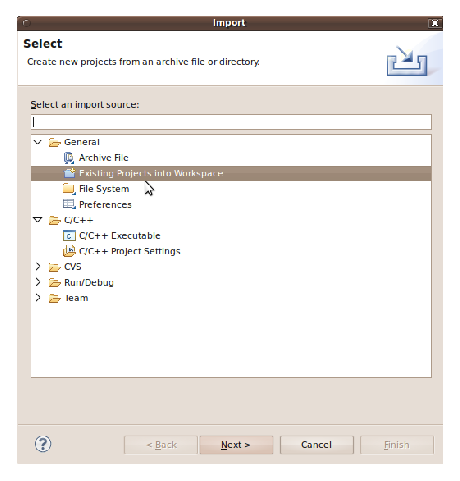
\includegraphics[scale=0.5]{pic/importexisting}}

\end{figure}
%
\begin{figure}[H]


\caption{Select ROSA directory or .zip package\protect \\
\protect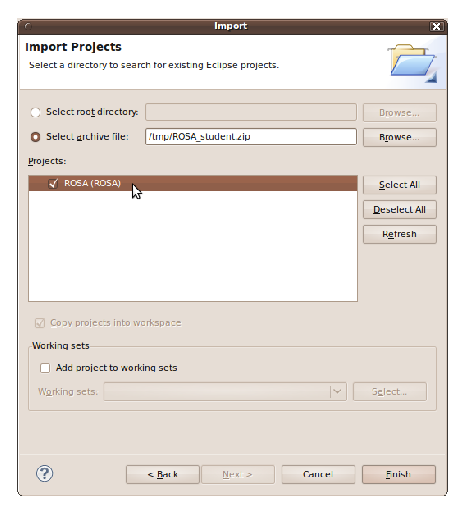
\includegraphics[scale=0.5]{pic/importexistingprojects}}



\end{figure}



\subsection{How to program ROSA\protect \\
onto the EVK1100}


\subsubsection{AVR32 Studio}

AVR32 Studio can also be used for programming the MCU flash by the
normal AVR32 Studio programming procedure. 


\section{ROSA kernel functionality}

This is a brief description of the kernel functionality.


\subsection{Kernel}

The ROSA kernel is the controller software and supervisor of the system.
As a user of ROSA you create and install {}``tasks'' into the ROSA
kernel. When ROSA is started one of the tasks is picked up and execution
is turned over to this task.

From time to time the task needs to give up its execution and let
other tasks run. The kernel perform a task context switch, thus allowing
the next waiting task to run.


\subsubsection{Kernel functions}

All kernel functions that the user can call are prefixed\emph{ ROSA\_},
e.g.\emph{ ROSA\_init().}

Part of the ROSA kernel is written in assembler. In order to be able
to share the same TCB structure from both assemebler and C the kernel
utilizes offsets found in the file rosa/src/include/kernel/rosa\_off.i.
These offsets are used by the assembler routines to access the elements
in the TCB block.


\subsubsection{Kernel configuration}

A few user configurations can be done through the\emph{ rosa\_config.h}
file. For example the timer period and the USART baudrate is defined
here. The default is 57600 baud.


\subsection{Task}

A task is a program running under the kernels supervision. A task
consists of:
\begin{itemize}
\item A TCB.
\item A data area.
\item Program code.
\end{itemize}

\subsubsection{TCB}

The TCB contain information and/or space for:
\begin{itemize}
\item Task identification (id/name).
\item Address to the next TCB in the TCB-list.
\item The start address of the task.
\item Where the data area is located and its size.
\item The current state, which is described by the return address and the
status register (SR).
\item All necessary CPU registers.
\end{itemize}
The exact definition of the TCB is found in the file rosa/src/include/kernel/rosa\_def.h.


\subsubsection{Data area}

The data area is the private stack for the task. The data area contains
temporary data etc. for the task. The stack size must be suitable
to hold all temporary data.


\subsubsection{Program code}

One of the important parts in a task is the program code. When the
kernel does a context switch the task program code starts to run.
The program code is executed in a never ending loop. From time to
time the program code call the kernel context switch function in order
to allow other tasks to run.


\subsection{TCBLIST}

The ROSA kernel utilizes a variable TCBLIST which contain a link to
the TCBs in the kernel. See Figure\ref{fig:Figure1tcblist}. Another
variable EXECTASK contains the TCB of the current executing task.

%
\begin{figure}[h]
\caption{TCBLIST is a circular linked list.\protect \\
\index{Figure1tcblist}\label{fig:Figure1tcblist}\protect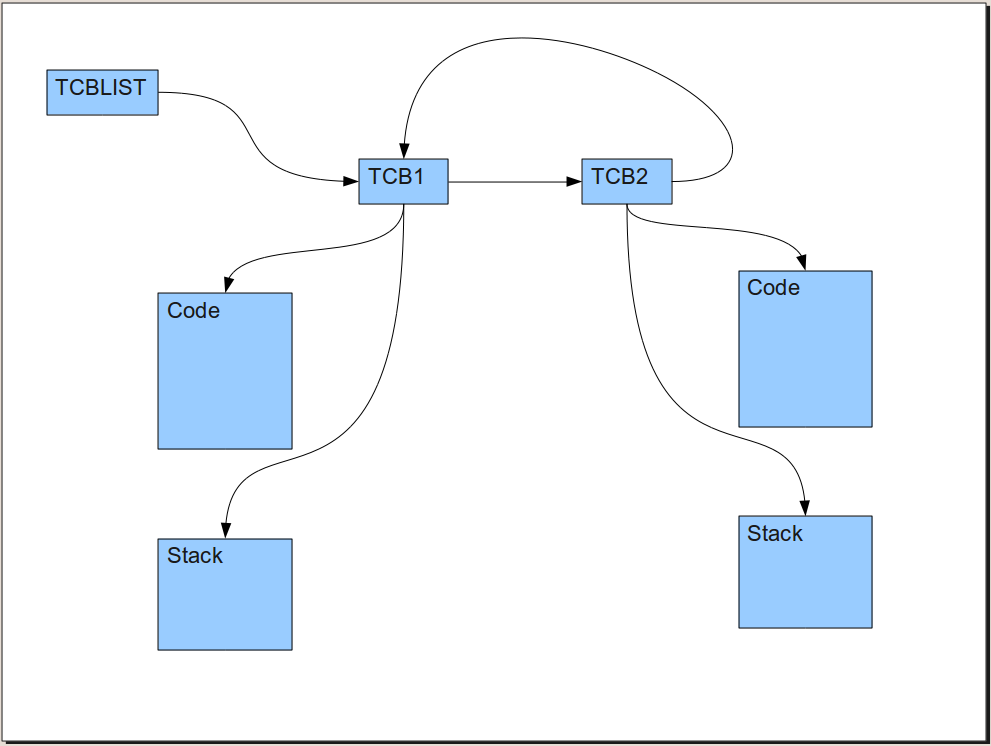
\includegraphics[scale=0.35]{pic/tcblist}}

\end{figure}



\section{The internal structure of ROSA}

This is a more detailed description of the internal structure of ROSA.

The first thing to note about ROSA is that kernel functions execute
in supervisor mode and the tasks execute in user mode. Mode switching
is done by ROSA.


\subsection{Creating and installing tasks}

All TCB's are linked together by the variable TCBLIST. When a task
have been created by\emph{ ROSA\_tcbCreate()} and installed in the
kernel by\emph{ ROSA\_tcbInstall()}, the TCBLIST will contain a reference
to the first TCB created.

When more tasks are created and installed, each TCB is linked into
the TCBLIST and the correct information is filled into the TCB.

These are the necessary informations that need to be initialized in
the TCB:
\begin{itemize}
\item How to find the next TCB.
\item Start and return address, the address the task will start execute
at.
\item The status register (SR) is set to work in user mode.
\item The user stack pointer (USP), which the task will use.
\item All CPU registers are saved into the TCB in order to not be destroyed
by a context switch.
\end{itemize}
Part of this needs to be done in assembler, due to the low level nature
of e.g. saving specific CPU registers. This is handled by the\emph{
contextInit()} call last in\emph{ ROSA\_tcbCreate()}.


\subsection{Starting the ROSA kernel}

When\emph{ ROSA\_start()} is called the first task in TCBLIST will
start to execute. In order to activate the first task we must load
the correct value for the user stack pointer (USP), and set the correct
value of the status register (SR). This needs to be done from assembler.

To start task execution the task start address, STADDR, is loaded
from the TCB and a jump is done to STADDR.


\subsection{Context switching}

When a task have finished its execution during a period,\emph{ ROSA\_yield()}
is called. The functionperforms the following sequence:
\begin{itemize}
\item The context of the CPU is stored to the TCB.
\item The scheduler function,\emph{ scheduler()}, is called and a new TCB
is written into EXECTASK. 
\item The context of the new TCB is restored by a call to\\
\emph{contextRestore()}.
\end{itemize}
The\emph{ ROSA\_yield()} utilizes the supervisor mode which is entered
by the '\emph{scall}' system call instruction. This instruction jumps
to the\emph{ \_handle\_Supervisor\_Call} vector and effectively runs
the context switch routines in supervisor mode.

%
\begin{figure}
\caption{The context switch procedure\protect \\
\protect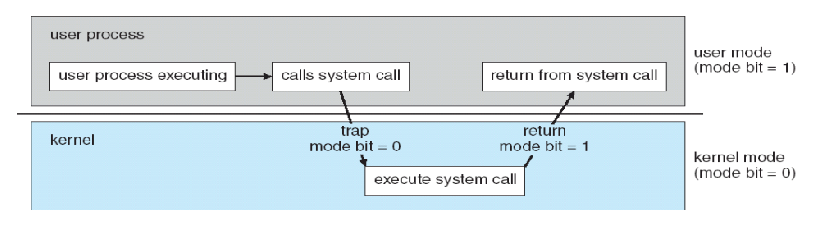
\includegraphics[scale=0.4]{pic/contextSwitch}}

\end{figure}



\subsubsection{Context save}

\emph{contextSave()} does the following operations:
\begin{itemize}
\item Fetch the TCB of the current executing task.
\item Saves temporary work registers.
\item Saves the status register, SR.
\item Saves the CPU registers.
\item Saves the return address.
\item Saves the correct user stack pointer, USP.
\end{itemize}

\subsubsection{Scheduling}

The\emph{ scheduler()} function fetch the next task to execute. The
currently running TCB, referenced to by the variable EXECTASK, is
changed to another TCB from the TCBLIST. A reference to the new task
TCB is put in the EXECTASK variable.


\subsubsection{Context restore}

\emph{contextRestore()} practically does the reverse of the context
save:
\begin{itemize}
\item Fetch the TCB from the EXECTASK.
\item Restores the USP.
\item Restores return address.
\item Restores CPU registers.
\item Restores SR.
\item Restores work registers.
\item Return from supervisor mode.
\end{itemize}
This sequence makes the CPU start executing the new task.


\section{How to use ROSA from C}

We will look at how ROSA can be used. The following code contains
two simple tasks and initialization of ROSA. Each task will control
LED1 and LED2 on the EVK1100.


\subsection{Simple source code walk through}

This is a description on how to set up the main.c file and start running
the ROSA kernel. A more detailed walk through of the kernel is found
in section\vref{sec:Kernel-source-code}


\subsubsection{Headers}

We start in the main.c by including the necessary header files.

%
\begin{framed}%

\begin{lstlisting}[basicstyle={\footnotesize\ttfamily},breaklines=true,language=C,showstringspaces=false,tabsize=4]
//Kernel includes
#include "kernel/rosa_ker.h"

//I/O driver includes
#include "drivers/led.h"
#include "drivers/delay.h"

//Include configuration
#include "rosa_config.h"
\end{lstlisting}
\end{framed}


\subsubsection{Tasks}

Now we define our tasks; task1 and task2. Note that the tasks consist
of a\emph{ while(1)}-loop, which basically will make the task run
forever.

The next thing to note is the\emph{ ledOn()/Off()} scheme, task1 will
light up LED1 of the EVK1100. Task2 will light up LED2. Pay attention
to the inconsistency between the labeling of the LEDs on EVK1100 and
the defined LEDx\_GPIO numbers.

\emph{ROSA\_yield()} is the function which performs a context switch,
allowing both tasks to run in pseudo parallel, despite the forever\emph{
while(1)}-loop.

%
\begin{framed}%

\begin{lstlisting}[basicstyle={\footnotesize\ttfamily},breaklines=true,language=C,showstringspaces=false,tabsize=4]
//TASK1
//--------------
//LED1 lights up
//LED2 goes dark
void task1(void)
{
	while(1) {
		ledOn(LED0_GPIO);	//EVK1100 LED1!
		ledOff(LED1_GPIO);
		ROSA_yield();
	}
}

//TASK2
//--------------
//LED2 lights up
//LED1 goes dark
void task2(void)
{
	while(1) {
		ledOff(LED0_GPIO);
		ledOn(LED1_GPIO);
		ROSA_yield();
	}
}
\end{lstlisting}
\end{framed}


\subsubsection{TCB and stack declaration}

We declare our TCB and stack for the two tasks we are going to create.
The first thing we do is to reserve stack space by defining a global
array with appropriate size. Space for the TCB is also reserved by
the tcb struct.

%
\begin{framed}%

\begin{lstlisting}[basicstyle={\footnotesize\ttfamily},breaklines=true,language=C,showstringspaces=false,tabsize=4]
//Data blocks for the tasks
#define T1_STACK_SIZE 0x40
static int t1_stack[T1_STACK_SIZE];
static tcb t1_tcb;

#define T2_STACK_SIZE 0x40
static int t2_stack[T2_STACK_SIZE];
static tcb t2_tcb;
\end{lstlisting}
\end{framed}


\subsubsection{More TCB and TCBLIST}

So far so good, but ROSA does not know where to find the tasks we
want to run, and neither are the TCBs of the tasks set up correctly
yet. This is done by calling\emph{ ROSA\_tcbCreate()} and\emph{ ROSA\_tcbInstall().}
This must be done before starting ROSA with the\emph{ ROSA\_start()}
call. Execution control is now in the hands of ROSA and will not return
to this point.

Below is an example of how it is done from the\emph{ main()}-function:

%
\begin{framed}%

\begin{lstlisting}[basicstyle={\footnotesize\ttfamily},breaklines=true,showstringspaces=false,tabsize=4]
int main(void)
{
	//Initialize ROSA
	ROSA_init();

	//Create tasks, set up the TCB correctly
	ROSA_tcbCreate(&t1_tcb, "tsk1", task1, t1_stack, T1_STACK_SIZE);
	ROSA_tcbCreate(&t2_tcb, "tsk2", task2, t2_stack, T2_STACK_SIZE);

	//Install the TCBs into the TCBLIST.
	ROSA_tcbInstall(&t1_tcb);
	ROSA_tcbInstall(&t2_tcb);

	//Start the ROSA kernel
	ROSA_start();
	/* Execution will never return here */
}
\end{lstlisting}
\end{framed}


\section{Kernel source code walk through\index{Kernel source code walk through}\label{sec:Kernel-source-code}}

This is a closer look at the ROSA kernel.

In the\emph{ main()} function, as shown previously, the first kernel
function to be called is\emph{ ROSA\_init().} This function sets the
TCBLIST and EXECTASK to NULL. This is done since no task have been
added yet. Also I/O is initialized by this function call.

%
\begin{framed}%

\begin{lstlisting}[basicstyle={\footnotesize\ttfamily},breaklines=true,language=C,tabsize=4]
void ROSA_init(void)
{
	//No tasks yet.
	TCBLIST = NULL;
	EXECTASK = NULL;

	//Do initialization of I/O drivers
	ledInit();                         //LEDs
	buttonInit();                      //Buttons
	joystickInit();                    //Joystick
	potInit();                         //Potentiometer
    usartInit(USART, &usart_options, FOSC0);//Serial
}
\end{lstlisting}
\end{framed}\medskip{}
Next the TCB's of two tasks are created by function call to\emph{
ROSA\_tcbCreate()}.

%
\begin{framed}%

\begin{lstlisting}[basicstyle={\scriptsize\ttfamily},tabsize=4]
ROSA_tcbCreate(&t1_tcb, "tsk1", task1, t1_stack, T1_STACK_SIZE);
ROSA_tcbCreate(&t2_tcb, "tsk2", task2, t2_stack, T2_STACK_SIZE);
\end{lstlisting}
\end{framed}\medskip{}
These calls fill in the necessary information into the TCB as shown
below. First the task id/name is copied into the TCB.

%
\begin{framed}%

\begin{lstlisting}[basicstyle={\footnotesize\ttfamily},breaklines=true,language=C,showstringspaces=false,tabsize=4]
void ROSA_tcbCreate(tcb * tcbTask, char tcbName[NAMESIZE],    void *tcbFunction, int * tcbStack, int tcbStackSize)
{
	int i;

	//Initialize the tcb with the correct values
	for(i = 0; i < NAMESIZE; i++) {
		//Copy the id/name
		tcbTask->id[i] = tcbName[i];
	}
\end{lstlisting}
\end{framed}\medskip{}
The link to the next TCB is set to NULL as this TCB block have not
been installed into the ROSA kernel yet.

%
\begin{framed}%

\begin{lstlisting}[basicstyle={\footnotesize\ttfamily},breaklines=true,language=C,showstringspaces=false,tabsize=4]
	//Dont link this TCB anywhere yet
	tcbTask->nexttcb = NULL;
\end{lstlisting}
\end{framed}\medskip{}
The start and return addresses are set up to point to the beginning
of the task function. The stack and its size are set up, and the USP
is set to point to the data area. An initial value of the SR is set.
This give us a known initial state of the task.

%
\begin{framed}%

\begin{lstlisting}[basicstyle={\footnotesize\ttfamily},breaklines=true,language=C,showstringspaces=false,tabsize=4]
	//Set the task function start and return address
	tcbTask->staddr = tcbFunction;
	tcbTask->retaddr = (int)tcbFunction;

	//Set up the stack
	tcbTask->datasize = tcbStackSize;
	tcbTask->dataarea = tcbStack + tcbStackSize;
	tcbTask->saveusp = tcbTask->dataarea;

	//Set the initial SR
	tcbTask->savesr = ROSA_INITIALSR;
\end{lstlisting}
\end{framed}\medskip{}
The last thing to do during TCB creation is to set up the task context
registers to a known state. This is done in assembler by the\emph{
context-Init()} call.

%
\begin{framed}%

\begin{lstlisting}[basicstyle={\footnotesize\ttfamily},breaklines=true,showstringspaces=false,tabsize=4]
	//Initialize context
	contextInit(tcbTask);
}
\end{lstlisting}
\end{framed}\medskip{}
The assembler routine initialize the lr register (task activation
record) to point to the start address, STADDR, of the task program
code. The registers in the TCB, TCB.SAVEREG.R0 - TCB.SAVEREG.R12,
are set to zero.

%
\begin{framed}%

\begin{lstlisting}[basicstyle={\footnotesize\ttfamily},breaklines=true,language=C,showstringspaces=false,tabsize=4]
contextInit:
	//Initialize lr in the savereg area
	ld.w r0,r12[TCB.STADDR]
	st.w r12[TCB.SAVEREG.LR],r0

	//Initialize regs to zero
	mov r0,0x0
	st.w r12[TCB.SAVEREG.R0],r0
	st.w r12[TCB.SAVEREG.R1],r0
	st.w r12[TCB.SAVEREG.R2],r0
	...
	st.w r12[TCB.SAVEREG.R12],r0
	mov pc,lr
\end{lstlisting}
\end{framed}\medskip{}


Now the TCB have been properly created and it is time to install the
TCB into the ROSA kernel.

%
\begin{framed}%

\begin{lstlisting}[basicstyle={\footnotesize\ttfamily},breaklines=true,language=C,showstringspaces=false,tabsize=4]
	//Install TCB into the TCBLIST.
	ROSA_tcbInstall(t1_tcb);
	ROSA_tcbInstall(t2_tcb);
}
\end{lstlisting}
\end{framed}\medskip{}
This function call checks to see if the TCBLIST is empty, which is
the case when t1\_tcb is installed. The TCB (t1\_tcb) is installed
at the first position of the list.

If the TCBLIST is not empty, which will be the case when t2\_tcb is
installed, the TCB will be attached to the last position in the list.

The TCBLIST is circular, which mean the last element will always point
to the first element.

%
\begin{framed}%

\begin{lstlisting}[basicstyle={\footnotesize\ttfamily},breaklines=true,language=C,showstringspaces=false,tabsize=4]
void ROSA_tcbInstall(tcb * tcbTask)
{
	tcb * tcbTmp;
	// Is this the first tcb installed?
	if(TCBLIST == NULL) {
		TCBLIST = tcbTask;

		//Install the first tcb
		TCBLIST->nexttcb = tcbTask;

		//Make the list circular
		tcbTask->nexttcb = TCBLIST;
	}
	else {
		//Find last tcb in the list
		tcbTmp = TCBLIST;
		while(tcbTmp->nexttcb != TCBLIST) {
			tcbTmp = tcbTmp->nexttcb;
		}

		//Install tcb last in the list
		tcbTmp->nexttcb = tcbTask;

		//Make the list circular
		tcbTask->nexttcb = TCBLIST;
	}
}
\end{lstlisting}
\end{framed}\medskip{}


Finally the ROSA kernel can be started:%
\begin{framed}%

\begin{lstlisting}[basicstyle={\footnotesize\ttfamily},breaklines=true,language=C,showstringspaces=false,tabsize=4]
	//Start the ROSA kernel
	ROSA_start();
	/* Execution will never return to here */
\end{lstlisting}
\end{framed}\medskip{}


In effect this is the initial context switch. This is an assembler
routine that sets EXECTASK to be the first task in the TCBLIST. The
routine loads information (USP, SR, STADDR, registers etc.) from EXECTASK
and puts it directly onto the processor.

Loading lr with STADDR means that we are going to continue execution
at the task program code when this routine is finished.

%
\begin{framed}%

\begin{lstlisting}[basicstyle={\footnotesize\ttfamily},breaklines=true,language=C,showstringspaces=false,tabsize=4]
ROSA_start:
	//Put the first task from TCBLIST into EXECTASK
	lda.w r12,TCBLIST
	lda.w r11,EXECTASK
	ld.w r12,r12[0x0]
	st.w r11[0x0],r12

	//Set up start USP
	ld.w r0,r12[TCB.SAVEUSP]
	st.w --sp,r0
	ldmts sp,sp
	ld.w r0,sp++

	//Load start lr, execution will jump here later
	ld.w lr,r12[TCB.STADDR]

	//Set up start SR, enter user mode
	ld.w r0,r12[TCB.SAVESR]
	mtsr 0x0,r0

	//Load start registers R0-R12
	ld.w r0,r12[TCB.SAVEREG.R0]
	ld.w r1,r12[TCB.SAVEREG.R1]
	ld.w r2,r12[TCB.SAVEREG.R2]
	...
	ld.w r12,r12[TCB.SAVEREG.R12]
	mov pc,lr
\end{lstlisting}
\end{framed}\medskip{}


Now task1 starts to execute. It will light LED1, turn LED2 off and
then immediately do a context switch.

%
\begin{framed}%

\begin{lstlisting}[basicstyle={\footnotesize\ttfamily},breaklines=true,language=C,showstringspaces=false,tabsize=4]
void task1(void)
{
	while(1) {
		ledOn(LED0_GPIO);	//EVK1100 LED1!
		ledOff(LED1_GPIO);
		ROSA_yield();
	}
}
\end{lstlisting}
\end{framed}\medskip{}
The context switch routine consists of switching to supervisor mode
and three calls to\emph{ contextSave(), scheduler()} and\\
\emph{contextRestore()}. When a call is done the return address
is written to the lr register. The lr register will be overwritten
by consecutive calls. Pushing the lr register to the stack is essential
as this contain the return address to the yielding task and needs
to be saved into the TCB.SAVEREG.LR in the \emph{contextSave} routine.

%
\begin{framed}%

\begin{lstlisting}[basicstyle={\footnotesize\ttfamily},breaklines=true,language=C,showstringspaces=false,tabsize=4]
ROSA_yield:
	pushm lr
	lda.w lr,_yield
	//Enter supervisor mode
	scall
_yield:
	call contextSave
	call scheduler
	call contextRestore
	//Execution will not return to here!
\end{lstlisting}
\end{framed}\medskip{}


The\emph{ contextSave()} routine saves the context from the processor
into the TCB of EXECTASK.

%
\begin{framed}%

\begin{lstlisting}[basicstyle={\footnotesize\ttfamily},breaklines=true,language=C,showstringspaces=false,tabsize=4]
contextSave:
	pushm r12
	//Fetch the current executing task
	lda.w r12,EXECTASK
	ld.w r12,r12[0x0]

	//Save work registers to TCB
	st.w r12[TCB.SAVER0],r0
	st.w r12[TCB.SAVER1],r1
	ld.w r0,sp++            	//Use r0 to save r12
	st.w r12[TCB.SAVEREG.R12],r0

	//Save task SR to TCB
	ld.w r0,sp[SF_SR]
	st.w r12[TCB.SAVESR],r0

	//Save task registers r0-r11 to TCB
	mov r0,TCB.SAVEREG.R11
	add r0,r12
	stmts r0,r0-r11

	//Get the address of the USP
	mov r0,sp
	st.w --sp,r0
	stmts sp,sp
	ld.w r1,sp++	//USP in r1

	//Save RETADDR to TCB
	ld.w r0,r1[SF_LR_TASK]

	//Get from user stack, return to task,
	//not to ROSA_yield
	st.w r12[TCB.RETADDR],r0

	//Save LR_task
	st.w r12[TCB.SAVEREG.LR],r0

	//Save USP
	sub r1,-0x04
	st.w r12[TCB.SAVEUSP],r1

	mov pc,lr
\end{lstlisting}
\end{framed}\medskip{}
When the scheduler is done a new task TCB is present in the EXECTASK.
Now\emph{ contextRestore()} will do the final part of the context
switch, i.e. turning execution over to the next task. Register values
are fetched from the TCB and written directly to the processor or
on the stack for retrieval when exiting supervisor mode.

%
\begin{framed}%

\begin{lstlisting}[basicstyle={\footnotesize\ttfamily},breaklines=true,language=C,showstringspaces=false,tabsize=4]
contextRestore:
	//Fetch the current executing task
	lda.w r12,EXECTASK
	ld.w r12,r12[0x0]

	//Restore USP
	ld.w r1,r12[TCB.SAVEUSP]
	st.w --sp,r1
	ldmts sp,sp
	ld.w r1,sp++

	//Restore LR = retaddr
	ld.w lr,r12[TCB.SAVEREG.LR]

	//Restore RETADDR
	ld.w r0,r12[TCB.RETADDR]
	st.w sp[SF_PC],r0

	//Restore registers
	mov r0,TCB.SAVEREG.R11
	add r0,r12
	ldmts r0,r0-r11

	//Restore r7
	ld.w r7,r12[TCB.SAVEREG.R7]

	//Restore SR
	ld.w r0,r12[TCB.SAVESR]
	st.w sp[SF_SR],r0			//Put SR on the stack for later fetch

	//Restore work registers
	ld.w r0,r12[TCB.SAVER0]
	ld.w r1,r12[TCB.SAVER1]
	ld.w r12,r12[TCB.SAVEREG.R12]

	//We are done, exit from supervisor mode
	rets
\end{lstlisting}
\end{framed}\medskip{}


Now execution is at task2, which will run until the\emph{ ROSA\_yield()}
turn over execution to the next task, which in this case is task1.

%
\begin{framed}%

\begin{lstlisting}[basicstyle={\footnotesize\ttfamily},breaklines=true,language=C,showstringspaces=false,tabsize=4]
void task2(void)
{
	while(1) {
		ledOff(LED0_GPIO);	//EVK1100 LED1!
		ledOn(LED1_GPIO);
		ROSA_yield();
	}
}
\end{lstlisting}
\end{framed}\medskip{}


The two tasks will continue to execute in this fashion, taking turn
to run their program code on the processor one loop at a time before
leaving execution over to the other task by the\emph{ ROSA\_yield()}
call.


\section{Summary}

We now know what parts are necessary to a small cooperative realtime
kernel. We have seen in detail how a simple system execute on the
ROSA kernel.
\end{document}
